\documentclass[a4paper, 9pt]{article}
%%%%%%%%%%%%%%%%%%%%%%%%%%%%%%%%%%%%%%%%%%%%%%%
%%%%%%%%%%%%%%%%%%%%%%%%%%%%%%%%%%%%%%%%%%%%%%%
% TO ANYONE READING THIS, THIS ASSIGNMENT STARTS OFF GREAT (ALL WORK IS ACCURATE) UP UNTIL PART 3, THEN ITS A CLUSTERFUCK%%%%%%%%%%% %%%%%%%%%%%%%%%%%%%%%%%%%%%%%%%%%%%%%%%%%%%%%%%
%%%%%%%%%%%%%%%%%%%%%%%%%%%%%%%%%%%%%%%%%%%%%%%
%%%%%%%%%%%%%%%%%%%%%%%%%%%%%%%%%%%%%%%%%%%%%%%
\usepackage{geometry}
 \geometry{
 a4paper,
 total={170mm,257mm},
 left=20mm,
 top=20mm,
 }
\usepackage{blindtext}
\usepackage{comment} % enables the use of multi-line comments (\ifx \fi) 
\usepackage{lipsum} %This package just generates Lorem Ipsum filler text. 
\usepackage{multirow}	
\usepackage{amssymb}
\usepackage{changepage}  
\usepackage{listings}
\usepackage{amsmath}
\usepackage{wrapfig}
\usepackage{mathpazo}
\include{macros}

\newcommand{\squarebk}[1]{\left[#1\right]}
\newcommand{\parenth}[1]{\left(#1\right)}
\newcommand{\curlies}[1]{ \left\{#1\right\} }
\newcommand{\fTWOspectral}[1]{ f_2(#1) }
\newcommand{\fkONE}{f_1(k)}
\newcommand{\dw}{d\omega}
\newcommand{\intREAL}{\int_\mathbb{R}}
\newcommand{\fkTWO}{f_2(\omega)}
\newcommand{\eitk}{\exp\left(i\tau k \right)}
\newcommand{\eitw}{\exp\left(i\tau \omega \right)}
\newcommand{\suminj}{\sum_{i=1}^{n_j}}
\newcommand{\rhoONE}{\rho_1(\tau)}
\newcommand{\rhoTWO}{\rho_2(\tau)}
\newcommand{\integ}{\int_\mathbb{R}}
\newcommand{\Gamnu}{\Gamma(\nu)}
\usepackage{graphicx}
\usepackage{subcaption}
\usepackage{listings}
\usepackage{bm}
\usepackage{bbm}
\usepackage{float}
\usepackage{bm}
\newcommand{\rhotau}{\rho(\tau)}
\newcommand{\rhoprime}{\rho '(\tau)}
\newcommand{\TwoNuMinusOne}{2^{\nu-1}}
\newcommand{\tauv}{\tau^\nu}

\newcommand{\Pmat}{\pmb{P}}
\newcommand{\PxminusPmu}{(\Pmat\xbold - \Pmat\mubold)}
\newcommand{\PxpiminusPmupi}{(\Pmat\xbold_\pi - \Pmat\mubold_\pi)}
\newcommand{\xpiminusmupi}{ (\pmb{x_{\pi}} - \pmb{ \mu_\pi })  }
\newcommand{\xbold}{ \pmb{x} }
\newcommand{\mupivec}{(\mu_{\pi_1}, ...,\mu_{\pi_1})}
\newcommand{\mubold}{ \pmb{\mu} }
\newcommand{\Sigbold}{ \pmb{\Sigma} }
\newcommand\tab[1][1cm]{\hspace*{#1}}
\newcommand{\norm}[1]{\left\lVert#1\right\rVert}
\newcommand\qtrtab[1][0.25cm]{\hspace*{#1}}
\newcommand{\Likelihood}{ (2\pi)^{-k/2} |\Sigbold|^{-1/2} \exp\left\{ -\frac{1}{2} (\xbold -\mubold)' \Sigbold^{-1} (\xbold - \mubold) \right\} }

\newcommand{\tauvMinusOne}{\tau^{\nu - 1}}
\newcommand{\PiLikelihood}{ (2\pi)^{-k/2} |\Sigbold_\pi|^{-1/2} \exp\left\{ -\frac{1}{2} (\xbold_\pi -\mubold_\pi)' \Sigbold_\pi^{-1} (\xbold_\pi - \mubold_\pi) \right\} }

\newcommand{\M}{ \mathcal{M} }
\newcommand{\xvec}{ {x_1,...,x_k} }
\newcommand{\xvecminus}{ {x_1,...,x_{k-1}} }
\newcommand{\pixvec}{ {x_{\pi_1},...,x_{\pi_k}} }
\newcommand{\subveckminus}{ _{s_1, ... , s_{k-1}} }
\newcommand{\subveckminusandk}{ _{s_1, ... , s_{k-1}, s_k} }
\newcommand{\subvec}{ _{s_1, ... , s_k} }
\newcommand{\pisubvec}{ _{s_{\pi_1}, ... , s_{\pi}} }
\newcommand{\ffunction}{ (x_1,...,x_k|\pmb{\mu}, \pmb{\Sigma}) }
\newcommand{\p}[1]{\left(#1\right)}
\newcommand{\bk}[1]{\left[#1\right]}
\newcommand{\bc}[1]{ \left\{#1\right\} }
\newcommand{\abs}[1]{ \left|#1\right| }
\newcommand{\mat}{ \begin{pmatrix} }
\newcommand{\tam}{ \end{pmatrix} }
\newcommand{\suml}{ \sum_{i=1}^N }
\newcommand{\prodl}{ \prod_{i=1}^n }
\newcommand{\ds}{ \displaystyle }
\newcommand{\df}[2]{ \frac{d#1}{d#2} }
\newcommand{\ddf}[2]{ \frac{d^2#1}{d{#2}^2} }
\newcommand{\pd}[2]{ \frac{\partial#1}{\partial#2} }
\newcommand{\pdd}[2]{ \frac{\partial^2#1}{\partial{#2}^2} }
\newcommand{\N}{ \mathcal{N} }
\newcommand{\E}{ \text{E} }
\newcommand{\V}{ \text{Var} }
\def\given{~\bigg|~}
\newcommand{\Poisson}{\text{Poisson}}
\def\gii{g^{-1}(x_i'\hat\beta)}
\def\mess{\frac{\exp(\beta_1+\beta_2 x_i)}{1+\exp(\beta_1+\beta_2 x_i)}}
\def\link{\exp(\beta_1 + \beta_2 x_i)}
\def\hier{Y_i | \beta_1, \beta_2, \lambda}
\def\M1{Y_i | \beta_1, \beta_2}
\newcommand{\Gam}{\text{Gamma}}

\title{AMS 207 - Homework 2}
\date{Mary Silva}
\author{Red Hawk Data}

\begin{document}
\maketitle
%Header-Make sure you update this information!!!!
% \noindent
% \textbf{AMS 201 Homework \#1} \hfill \textbf{Mary Silva}\\
% UCSC \hfill  26 April 2019\\


Write the Bayes factor, BIC, DIC and Gelfand and Ghost criterion to compare a model where n observations are assumed to be sampled with a poisson distribution with a gamma prior, to a model where the observations are sampled from a binomial distribution, with a fixed, large, number of trials and beta prior for the probability of success.

\begin{enumerate}
\item[1.] Consider the data on red tailed hawks. Fit the data using the two different models. Notice that there is no hierarchical structure in this case, as opposed to what was assumed in the take home part of Test 1. Ignore the route counts.\\
\\

We first fit the data using a Poisson distribution with a Gamma prior:
\begin{align*}
    M_1 :& X_i \sim \Poisson (\lambda); \tab i=1,...,n\\
        &\lambda \sim Gamma(\alpha, \beta)
\end{align*}
The likelihood for model 1 is given by:
\begin{align*}
    f_1(\pmb{x}|\lambda) = \frac{e^{-n\lambda}\lambda^{\sum x_i}}{\prod x_i!} 
\end{align*}
The prior for model 1 is given by
\begin{align*}
    \pi(\lambda) =\frac{\beta^\alpha}{\Gamma(\alpha)}\lambda^{\alpha - 1} \exp{-\lambda \beta}
\end{align*}
Which leads to the following posterior
\begin{align}
    \pi_1(\lambda|\pmb{x}) &\propto f(\pmb{x}|\lambda) p(\lambda)\\
    &\propto \frac{\beta^\alpha}{\Gamma(\alpha) \prod x_i!}\exp\Big\{-\lambda(n+\beta)\Big\}\lambda^{\sum x_i + \alpha-1}\\
\end{align}
Which we recognize as the kernel of a Gamma distribution. Thus, 
\begin{align}
    \lambda|\xbold \sim & \sim Gamma\left(\alpha^{*} = \sum x_i + \alpha, \beta^{*} = n + \beta\right)
\end{align}

For the second model, we fit the data using a binomial distribution with a fixed, large number of trials and a beta prior
\begin{align*}
    M_2:& X_i \sim Binom(n,\theta); \tab i=1,...,n\\
    & \theta \sim Beta(\alpha,\beta)
\end{align*}

The Likelihood:
\begin{align*}
    f_2(\pmb{x}|\theta) = \prod_{i=1}^{n} {{N}\choose{x_i}} \theta^{\sum x_i}(1 - \theta)^{nN - \sum x_i}
\end{align*}

The prior:
\begin{align*}
\pi(\theta) = \frac{\Gamma(\alpha + \beta)}{\Gamma(\alpha)\Gamma(\beta)}\theta^{\alpha - 1} (1 - \theta)^{\beta - 1}
\end{align*} 
Throughout this paper, I use large $N = 10^6$.\\
The posterior distribution for model 2 up to a constant is:
\begin{align}
    \pi_2(\lambda|\pmb{x}) &\propto \left[ \prod_{i=1}^{n} {{N}\choose{x_i}}\right]\frac{\Gamma(\alpha + \beta)}{\Gamma(\alpha)\Gamma(\beta)} \theta^{\sum x_i +  \alpha - 1} (1-\theta)^{nN + \beta - \sum x_i -  1}
\end{align}
Which we recognize as the kernel for Beta distribution, therefore
\begin{align}
    \theta|\xbold \sim Beta\left(\alpha^* = \sum x_i + \alpha, \beta^* = nN + \beta - \sum x_i\right)
\end{align}


\item[2.] Perform a prior sensitivity analysis.\\
\\
We are going to explore various non-informative and informative priors for both models. For model $M_1$, as an informative prior, we want to choose $\alpha$ and $\beta$ such that the prior mean, $E(\lambda) = \frac{\alpha}{\beta}$, is proportional to the maximum likelihood estimator $\hat\lambda = \text{mean(data)} = 376.1$. So we will set $\alpha = 376.1$ and $\beta = 1$ as our informative prior and compare to weakly informative priors (Figure \ref{GammaCompare}). We plot the posterior distributions using different $\alpha$ and $\beta$ values and attaining the $\alpha^*$ and $\beta^*$ values obtained in equation (4). 
\\\\\\

\begin{figure}[h!]
    \centering
    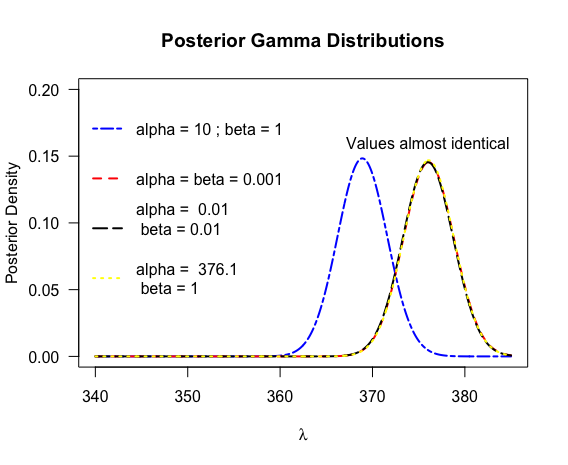
\includegraphics[scale = 0.6]{GammaPost.png}
    \captionsetup{width=.6\linewidth}
    \caption{Posterior densities for $\lambda|\xbold \sim Gamma(\alpha^*, \beta^*)$. We see that the posterior distribution for model 1 is not sensative to prior selection when the prior mean is centered around the MLE.}
    \label{GammaCompare}
\end{figure}

Similarly, for model $M_2$, we want to select informative priors $\alpha$ and $\beta$ for the Beta distribution so that the prior mean is proportional to the MLE. In other words, we want the prior mean to be centered around $376.1/N =$ {3.761e-04} (Figure \ref{BetaPost}). We note that, based on the plot, prior selection makes very little difference for the second model.

\begin{figure}[h!]
    \centering
    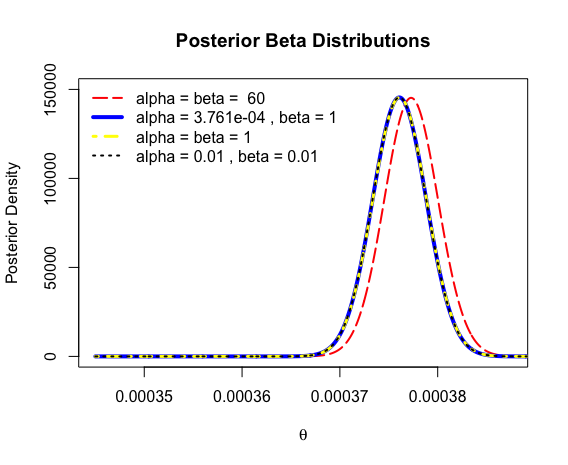
\includegraphics[scale = 0.6]{BetaPost.png}
    \captionsetup{width=.6\linewidth}
    \caption{Posterior densities for $\theta|\xbold \sim Beta(\alpha^*, \beta^*)$. We see that the posterior distribution for model 1 is not sensative to prior selection, thus any of the above priors would be justified in using.}
    \label{BetaPost}
\end{figure}

\item[3.] With $n$ being the number of red tailed hawk observations, we define the following criterion:\\
\\
\subsection*{BIC}
$$BIC = -2 \times \text{Likelihood} - \log(n)$$
\subsection*{DIC}
For the Deviance Information Criterion (DIC), the deviance statistic is given by
$$D(\theta) = -2 \log \text{Likelihood} + 2 \log{h(x)}$$
where $h(x)$ is the standardizing function. Then the DIC is given by
$$DIC = \Bar{D} + (\Bar{D} - D(\Bar{\theta})) = 2 \Bar{D} - D(\Bar{\theta})$$
Where $D(\Bar{\theta})$ is the mean of posterior samples.
\\
\\
\subsection*{Gelfand and Ghosh}
For the Gelfand and Ghosh criterion, denote the observed data as $\xbold$ and $z$ as the new predicted value given x. Therefore we have the following posterior predictive distribution for 

\begin{align*}
    M_1: p_1(z|\xbold) &= \int_{0}^\infty f_1(z|\lambda) \pi_1(\lambda|\xbold)d\lambda\\
    & = \frac{\Gamma(z + \sum x_i + \alpha)}{\Gamma(\sum x_i + \alpha) \Gamma(z+1)}\parenth{\frac{n+\beta}{n+\beta + 1}}^{\sum x_i + \alpha} \parenth{\frac{1}{n + \beta + 1}}^z
\end{align*}

Which is a negative binomial distribution with mean
$$ \frac{\sum x_i + \alpha}{n+\beta}$$
and variance
$$\frac{\sum x_i + \alpha}{(n+\beta)^2}(n+\beta+1) $$

The posterior predictive distribution for model 2 is
\begin{align*}
    M_2: p_2(z|\xbold) & = \int_0^1 f_2(z|\theta)\pi_2(\theta|x)d\theta\\
    &= {N\choose{z}} \frac{Beta(z + \alpha_0^*, n -z + \beta_0^*)}{Beta(\alpha_0^*, \beta_0^*)}
\end{align*}

where $$\alpha_0^* = \sum x_i + \alpha$$ 
and 
$$\beta_0^* = nN + \beta - \sum x_i$$
We recognize this as a Beta-Binomial distribution with mean
$$\frac{N\alpha_0^*}{\alpha_0^* + \beta_0^*} $$
and variance
$$\frac{N\alpha_0^* \beta_0^* (\alpha_0^* + \beta_0^* + n)}{(\alpha_0^* + \beta_0^*)^2(\alpha_0^* + \beta_0^* + 1)}$$

(Sorry, there's a lot of alphas and betas going on around here, its getting ugly; but Wikipedia, am I right?)

% \textbf{x} and z as replicates of the observed data. Let $\mu_l = E(z_l| \pmb{x})$ and $\sigma^2_l = Var(z_l| \pmb{x})$
% For the Gelfand and Ghosh criterion, denote the observed data as
% \textbf{x} and z as replicates of the observed data. 

Let $\mu_l = E(z_l| \pmb{x})$ and $\sigma^2_l = Var(z_l| \pmb{x})$. Then the Gelfand and Ghosh criterion is given by

$$D = G + P,$$ 
where $$G=\displaystyle \sum_l (\mu_l - x_l)^2$$
and 
$$P = \displaystyle \sum_l \sigma^2_l$$

D seeks to reward goodness of fit penalizing complexity. So the smaller the D the better.

%We note that the posterior predictive distribution has closed form






\subsection*{Bayes Factor}
Next we look at the Bayes factor, which is simply a ratio of the marginals for model 1 and model 2.
\\
\\
Here we compute the marginals:
\begin{align}
m_1(x) &= \int f_1(x|\lambda) p_1(\lambda)d\lambda\\
&= \frac{\beta^\alpha}{\Gamma(\alpha) \prod (x_i!)} \int e^{-\lambda(n + \beta)} \lambda^{\sum x_i + \alpha - 1}d\lambda\\
&= \frac{\beta^\alpha}{\Gamma(\alpha) \prod (x_i!)} \frac{\Gamma(\sum x_i + \alpha)}{(n + \beta)^{\sum x_i + \alpha}}
\end{align}

\begin{align}
    m_2(x) &= \int f_2(x|\lambda) p_2(\lambda)d\lambda\\
    &=\left[ \prod_1^{n} {{N}\choose{x_i}}\right]\frac{\Gamma(\alpha + \beta)}{\Gamma(\alpha)\Gamma(\beta)} \int \theta^{\sum x_i  \alpha - 1} (1-\theta)^{nN + \beta - \sum x_i -  1}\\
    &=\left[ \prod_1^{n} {{N}\choose{x_i}}\right]\frac{\Gamma(\alpha + \beta)}{\Gamma(\alpha)\Gamma(\beta)} \frac{\Gamma(\sum x_i + \alpha) \Gamma(nN + \beta - \sum x_i)}{\Gamma(\alpha +nN + \beta)}
\end{align}

To calculate the Bayes factor, we use our previously defined $\alpha$ and $\beta$ parameters from part 2, and compute the ratio of the log marginals and then exponentiate the value.
$$\text{Bayes Factor} = \exp\{\log m_1 - \log m_2\} = 0.82 $$
Our Bayes factor is close to 1, therefore there is no real evidence in favor of either model over the other.

\subsection*{Criterion Summary/Conclusions}

We provide a table specifying our R calculations with using the informative priors previously specified.


\begin{table}[h!]
\centering
\begin{tabular}{rrrrl}
  \hline
 & BIC & DIC & Gelfand and Ghosh & Bayes Factor \\ 
  \hline
M1 & 2124.45 & 2122.52 & 549018.3 & 0.82 \\ 
  M2 & 2124.98 & 2123.03 & 549019.5 &          \\ 
  Difference & 0.53 & 0.51 & 1.17 &          \\ 
   \hline
\end{tabular}
\end{table}

\end{enumerate}

From the table, we see that the BIC, DIC, and G\&G criterion are slightly smaller for model 1 (the gamma posterior model). This implies that model 1 is the ``better" model. But in this case since the difference is slight, so we conclude that for model 2 (the beta posterior model) when we use a fixed, large, number of trials for the binomial prior as we have done, both model 1 and model 2 are essentially equivalent in terms of fitting the data, which is to be expected.



\end{document}
